\section{Related Work}
\label{sec:related-work}

Our work uses the data collected by Zhaohui Che, Ali Borji, Guangtao Zhai, Xiongkuo Min, Guodong Guo, and Patrick Le Callet \cite{gaze-transformations}, who studied 18 common digital image transformations shown in \Cref{transformations} and \Cref{cropping}. The dataset consists of 100 randomly selected images from the CAT2000 dataset \cite{cat2000}, with measured gaze distributions for the untransformed and the 18 transformations of each image.

The study by Che \etal \cite{gaze-transformations} aims to find transformations to augment data sets, but they make tangential analyses and comparisons between the gaze distributions of the transformations they study. Their analysis shows that transformations can affect gaze behavior in nontrivial ways.

\begin{figure}[t]
    \centering
    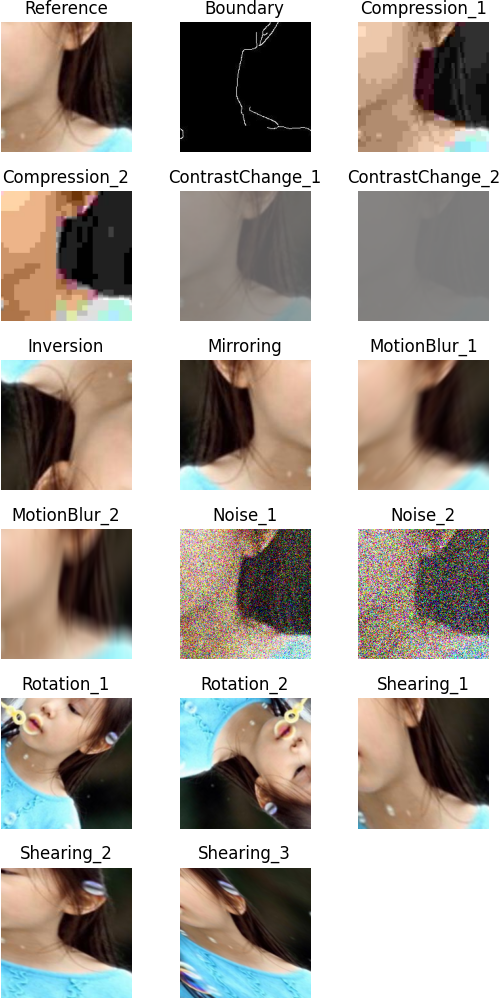
\includegraphics[width=0.8\linewidth]{figures/transformation_examples.png}
    \caption{Demonstrations of all transformations except \texttt{Cropping\char`_1} and \texttt{Cropping\char`_2}, which are shown in Figure 2. A slice of the first image in the dataset is shown, where both the untransformed slice and all transformations of the slice are displayed with transformation type labeled above each.}
    \label{transformations}
\end{figure}

\begin{figure}[t]
    \centering
    \begin{subfigure}{0.45\linewidth}
        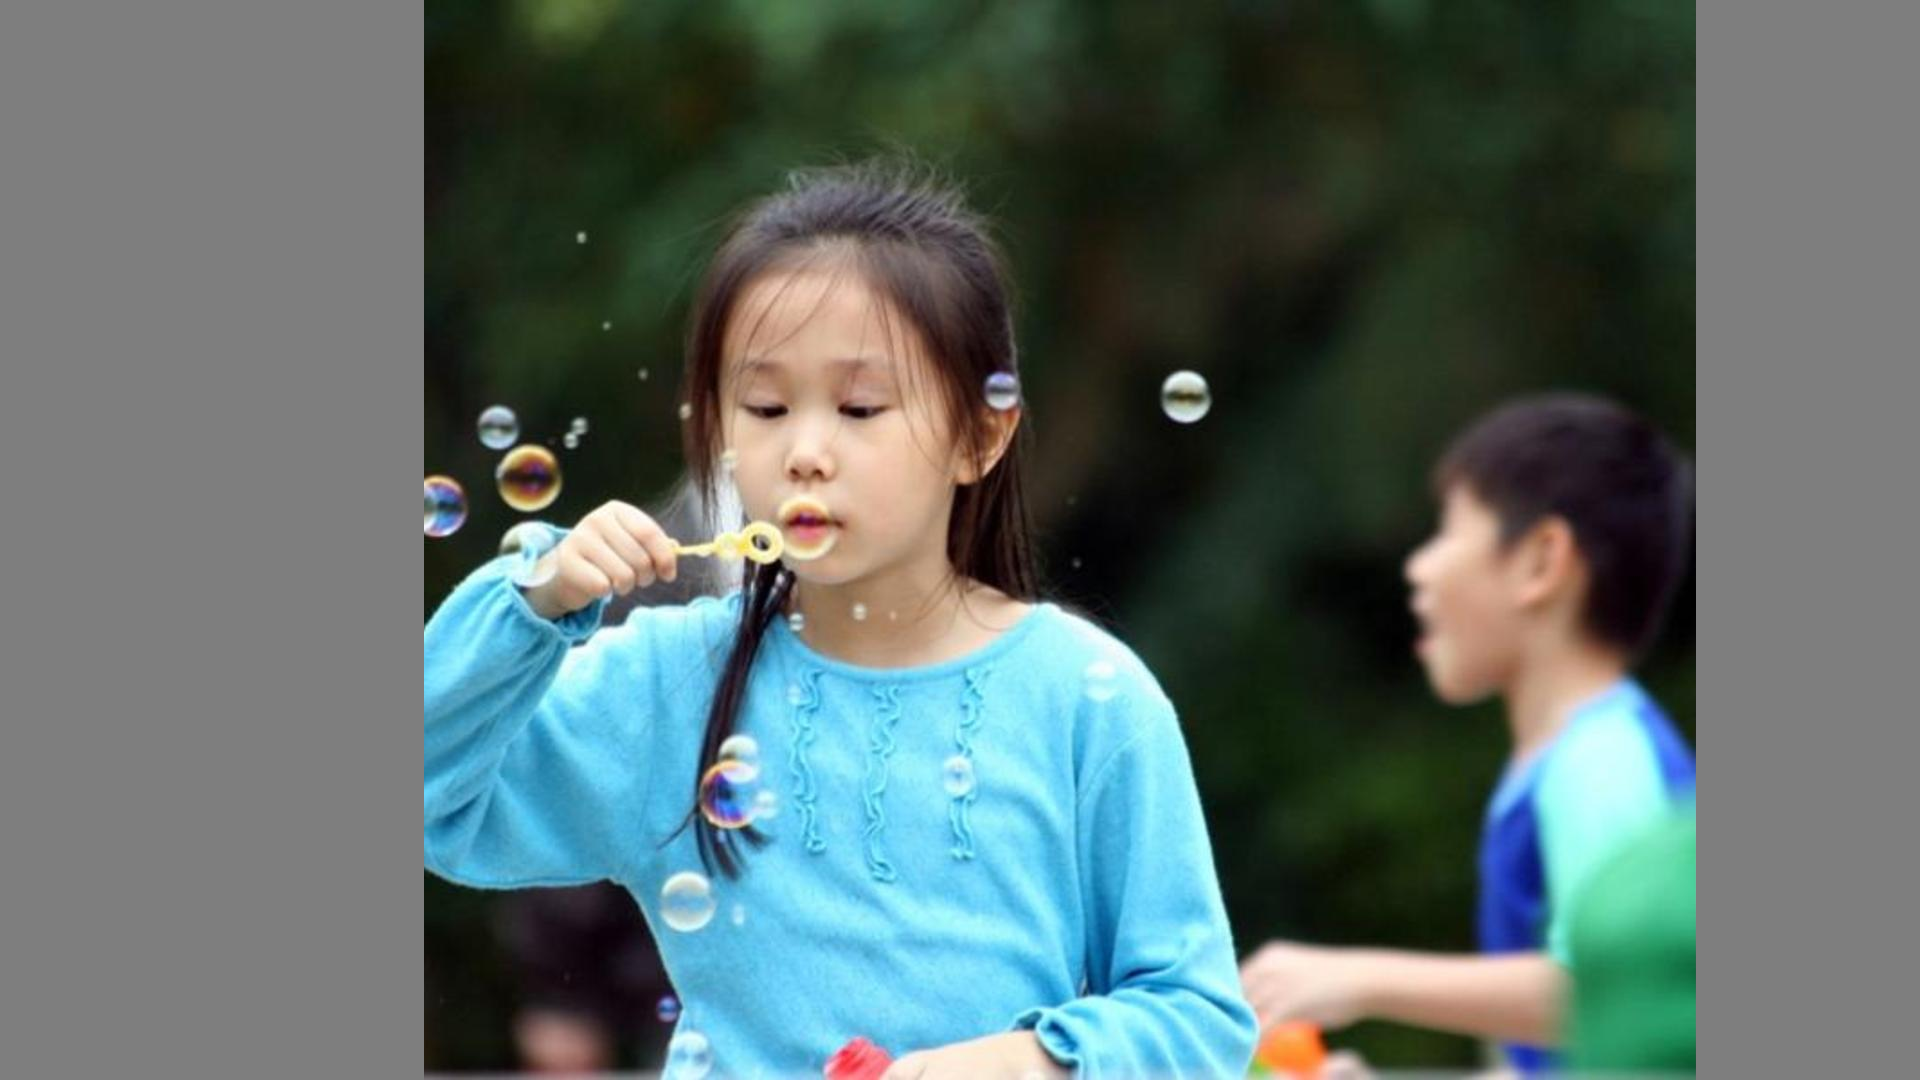
\includegraphics[width=1\linewidth]{figures/cropping_1_example.png}
    \end{subfigure}
    \hfill
    \begin{subfigure}{0.45\linewidth}
        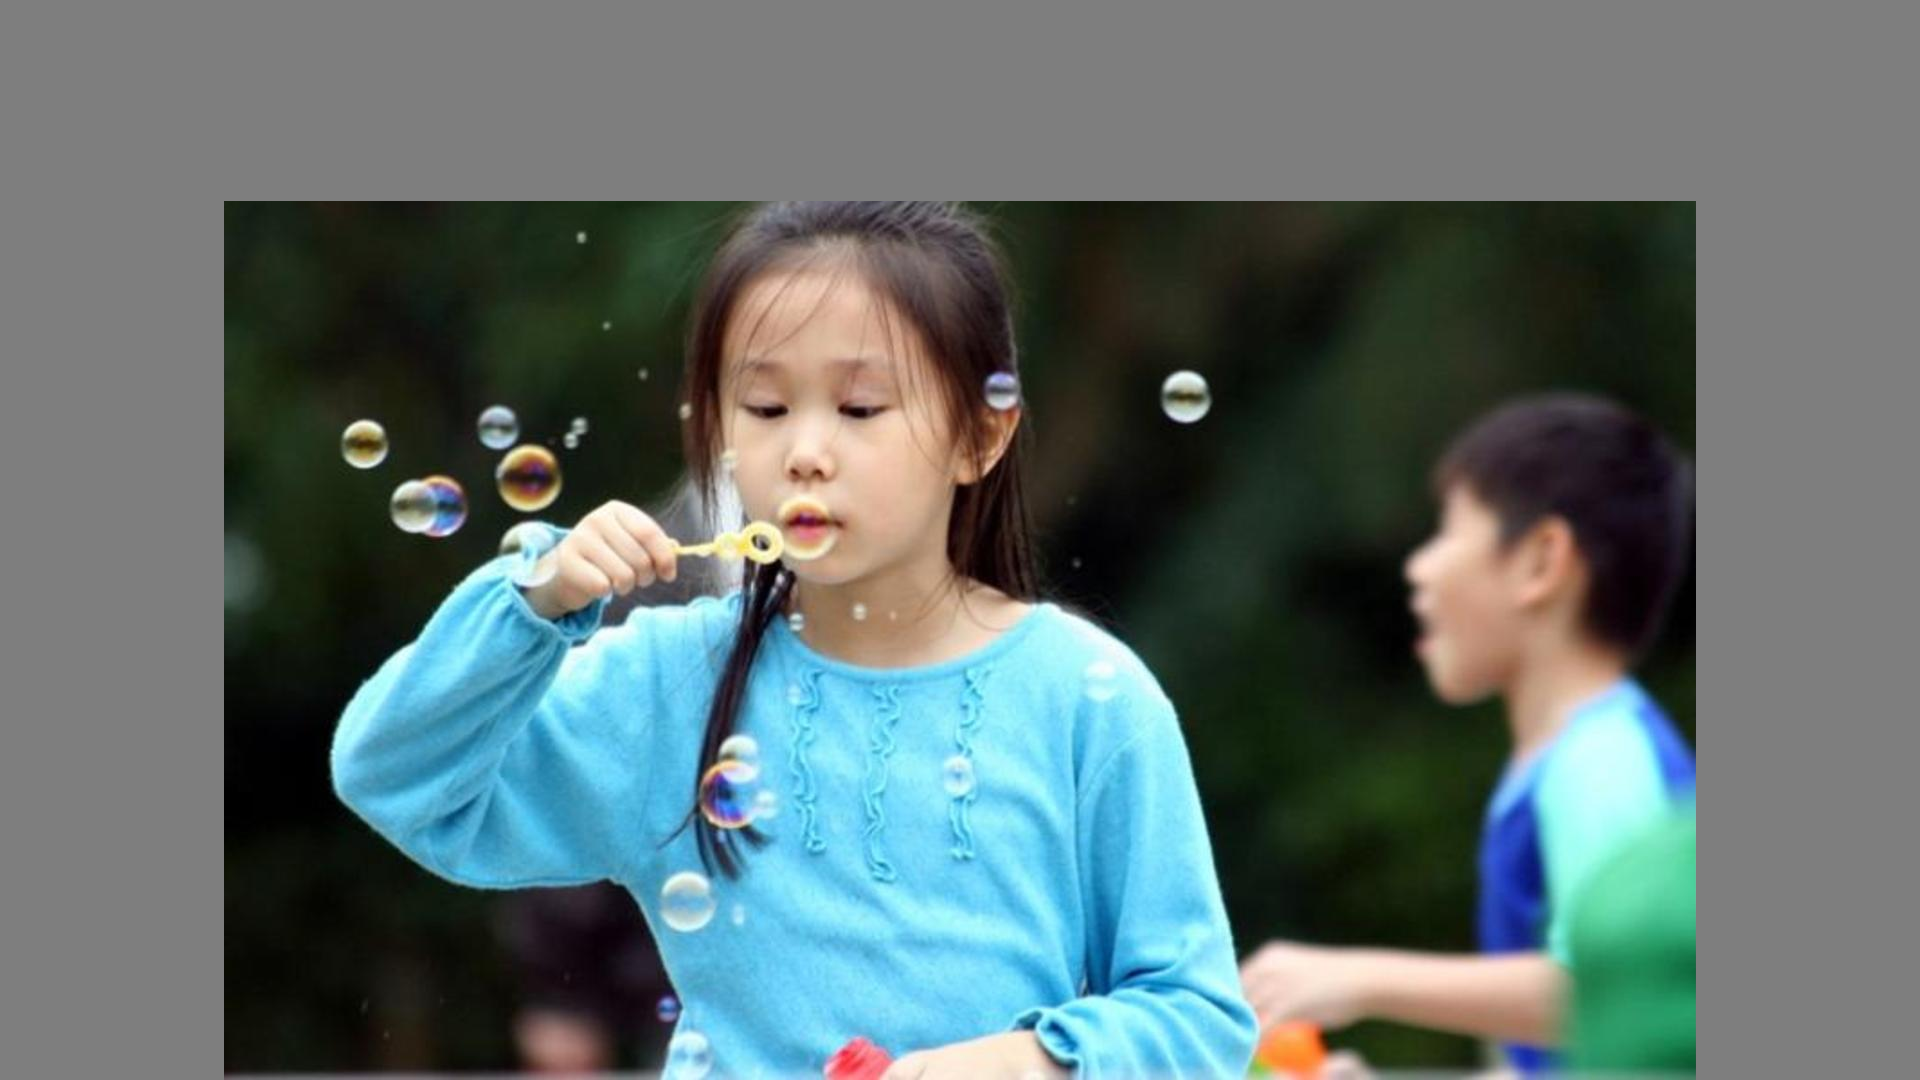
\includegraphics[width=1\linewidth]{figures/cropping_2_example.png}
    \end{subfigure}
    \caption{Demonstrations of \texttt{Cropping\char`_1} and \texttt{Cropping\char`_2} transformations on the left and right respectively.}
    \label{cropping}
\end{figure}

Our study builds on their work by computing the predictions of state-of-the-art models for the transformations they study, and then comparing those predictions to the gaze distribution data they collected for those transformations. Our work checks whether gaze prediction models can capture the nontrivial transformations of gaze behavior Che \etal \cite{gaze-transformations} describe.

The effects of digital image alterations on gaze behavior have also been studied by Rodrigo Quian Quiroga and Carlos Pedreira \cite{quianquiroga}, who performed an experiment collecting gaze fixations before and after manual Photoshop edits were made to photographs of paintings. Insufficient explanation for the intention behind edits makes it difficult to formally and generally describe the image transformations they studied. Instead, we study more common image transformations that have been applied consistently across a greater scale of data.

The effect of adversarial digital image transformations have been tested for both humans and deep learning models for the object recognition task by Girik Malik, Dakarai Crowder, and Ennio Mingolla \cite{object-recognition-transforms}. In contrast to their work, our experiments and datasets are designed for the gaze recognition task, a closely related but distinct domain. They test on variations of a pixel-shuffling algorithm, while we test cropping, rotation, skewing, edge detection, and other transformations more commonly seen in visual media applications.